\documentclass[11pt,a4paper]{article}

% ====== Paquetes base ======
\usepackage[utf8]{inputenc}
\usepackage[T1]{fontenc}
\usepackage[spanish,english]{babel} % Elige el idioma principal abajo
\selectlanguage{spanish}

\usepackage{lmodern}
\usepackage{geometry}         % Márgenes
\geometry{margin=2.5cm}

\usepackage{setspace}         % Espaciado
\onehalfspacing

\usepackage{graphicx}         % Imágenes
\graphicspath{{figures/}}     % Carpeta por defecto para figuras
\usepackage{booktabs}         % Tablas bonitas
\usepackage{multirow}
\usepackage{siunitx}          % Alineación de números en tablas
\sisetup{detect-all}
% Control fino de flotantes y barreras
\usepackage{float}     % habilita [H]
\usepackage{placeins}  % habilita \FloatBarrier


\usepackage{amssymb}

\usepackage{amsmath,amssymb}  % Matemáticas
\usepackage{hyperref}         % Enlaces
\hypersetup{
  colorlinks=true,
  linkcolor=blue,
  citecolor=blue,
  urlcolor=blue
}

\usepackage{caption}
\usepackage{subcaption}

% ====== Bibliografía con biblatex ======
\usepackage[
  backend=biber,
  style=apa,       % puedes usar numeric, ieee, authoryear, etc.
  sorting=nyt,
  natbib=true
]{biblatex}
\addbibresource{bib/references.bib}



\usepackage{booktabs,siunitx,tabularx,makecell}


\begin{document}
\begin{titlepage}
  \thispagestyle{empty}
  \centering

  \vspace*{\fill} % empuja desde arriba

  {\Huge \textbf{Explainable AI – Unidad 2: Árbol de Decisión (Primera Entrega)}\par}
  \vspace{1cm}

  {\Large
  Josep Gabriel Fornes Reynes\\
  Jordi Florit Ensenyat\\
  Juan Esteban Rincón Marín\par}

  \vspace{1.2cm}

  {\large Septiembre 2025\par}

  \vspace*{\fill} % empuja hacia abajo
\end{titlepage}

\clearpage

% ====== Secciones (organizadas en /sections) ======
\section{Introducción}

\paragraph{Resumen del problema y enfoque}

El objetivo de esta entrega es entrenar y explicar un modelo \de árbol de decisión para predecir la variable \texttt{recid}. El flujo de trabajo es sencillo para esta entrega es sencillo: EDA breve para identificar características de los datos, preprocesamiento encapsulado en \texttt{Pipeline} con \texttt{ColumnTransformer}, un primer modelo \emph{baseline} sin ajuste y un segundo modelo con los hiperpaámetros ajustados mediante \texttt{GridSearch}. Al final se presentan los resultados de ambos modelos y se estduia la explicabilidad global y local del modelo ajustado.

\paragraph{Datos (características y procesamiento)}
Trabajamos con el conjunto \texttt{recidivism.csv}, con \texttt{recid} como variable objetivo (binaria) y el resto de variables numéricas y categóricas. El EDA se centra en calidad de datos (nulos, cardinalidad) y equilibrio de clases (proporciones e \emph{Imbalance Ratio} de \textbf{1.14}). El preprocesamiento separa variables numéricas (\emph{passthrough}) y categóricas (codificación One-Hot), todo dentro de un \texttt{Pipeline} para evitar \emph{leakage} y garantizar que las mismas transformaciones se apliquen en validación y test.

\paragraph{Resultados (visión general)}
El \emph{baseline} sin ajuste alcanza \(\sim\)0.66 de \emph{accuracy} en validación. Tras el \texttt{GridSearch}, el mejor árbol obtiene en test \(\sim\)0.70 de \emph{accuracy} y mejora de forma consistente las métricas por clase (\textbf{precision}, \textbf{recall} y \textbf{F1}). Además, el ajuste produce un modelo más \textbf{explicable a nivel global}: el árbol es más compacto (menor profundidad y menos reglas), se puede \emph{pintar} y recorrer con claridad, y facilita la extracción de reglas comprensibles; a nivel local, las rutas de decisión son más cortas y fáciles de justificar.




\section{Metodología}

\subsubsection{Árbol baseline (referencia)}
Como primer paso se entrena un \texttt{DecisionTreeClassifier} con parámetros por defecto dentro del \texttt{Pipeline}. Este modelo sirve como modelo de referencia para responder a dos preguntas: (i) si la representación y el preprocesado son adecuados (el árbol aprende patrones sin necesidad de ingeniería adicional), y (ii) cuánto aporta realmente el ajuste de hiperparámetros. La elección de un árbol como baseline se justifica por su \textbf{transparencia inmediata} (reglas y estructura legibles) y por su bajo coste computacional.

\subsubsection{Árbol ajustado (GridSearchCV)}
En un segundo paso se ajusta el mismo clasificador mediante \texttt{GridSearch} con validación cruzada (5 particiones). La rejilla explora hiperparámetros que controlan el compromiso sesgo–varianza y la legibilidad del árbol:

\begin{itemize}
  \item \textbf{\texttt{max\_depth}}: limita la profundidad para reducir sobreajuste.
  \item \textbf{\texttt{min\_samples\_leaf}} y \textbf{\texttt{min\_samples\_split}}: evitan hojas muy pequeñas, estabilizando reglas y mejorando la generalización.
  \item \textbf{\texttt{criterion} (gini, entropy, log\_loss}: distintos criterios de división; \texttt{log\_loss} tiende a probabilidades más informativas, \texttt{gini}/\texttt{entropy} suelen ser más rápidos.
  \item \textbf{\texttt{max\_features} (None, sqrt, log2)}: puede actuar como regularizador al limitar atributos por división; en un único árbol se prioriza la \textbf{determinación} y legibilidad (\texttt{None}) salvo que limitarlo mejore validación.
  \item \textbf{\texttt{splitter} (best, random)}: \texttt{best} ofrece divisiones deterministas y normalmente mejores; \texttt{random} solo si se busca explorar particiones alternativas.
\end{itemize}

\paragraph{Configuración ganadora.}
Conforme al criterio de selección empleado, la mejor configuración obtenida fue:

\begin{table}[h]
\centering
\label{tab:best-params}
\small
\begin{tabular}{@{}ll@{}}
\toprule
\textbf{Parámetro}              & \textbf{Valor} \\ \midrule
\texttt{criterion}              & \texttt{gini} \\
\texttt{max\_depth}             & \texttt{3} \\
\texttt{min\_samples\_leaf}     & \texttt{1} \\
\texttt{min\_samples\_split}    & \texttt{2} \\
\texttt{max\_features}          & \texttt{None} \\
\texttt{class\_weight}          & \texttt{None} \\
\texttt{splitter}               & \texttt{best} \\ \bottomrule
\end{tabular}
\caption{Hiperparámetros óptimos devueltos por \texttt{GridSearchCV}.}
\end{table}
% Sustituir los <rellenar> por los valores que devuelve GridSearchCV.best_params_

Esta configuración \textbf{mejora} las métricas de evaluación frente al baseline (precision, recall y F1 por clase) y, al imponer \texttt{max\_depth} y un \texttt{min\_samples\_leaf} menor, produce un árbol \textbf{más compacto y explicable}: menos nodos/hojas, reglas más cortas y un diagrama del árbol que se puede \emph{pintar} y recorrer con claridad.


\section{Resultados}

\begin{table}[h]
\centering
\label{tab:results-summary}
\scriptsize
\setlength{\tabcolsep}{4pt}
\sisetup{table-format=1.3}
\begin{tabularx}{\linewidth}{@{}l X S S@{}}
\toprule
\textbf{Classifier} & \textbf{Best parameters} & {\textbf{Train acc}} & {\textbf{5-fold CV accuracy}} \\
\midrule
DecisionTree (baseline) &
\textit{defaults} &
0.670 & 0.659 \\

DecisionTree (tuned) &
\makecell[tl]{\texttt{criterion=gini, max\_depth=3,}\\
\texttt{min\_samples\_leaf=1, min\_samples\_split=2,}\\
\texttt{max\_features=None, class\_weight=None,}\\
\texttt{splitter=best}} &
0.700 & 0.719 \\

LogisticRegression &
\makecell[tl]{\texttt{C=1.0, penalty='l2', solver='lbfgs'}} &
0.732 & 0.702 \\

ExplainableBoostingMachine (GAM) &
\makecell[tl]{\texttt{learning\_rate=0.05, max\_bins=256,}\\
\texttt{interactions=5}} &
0.748 & 0.723 \\
\bottomrule
\end{tabularx}
\caption{Resumen de resultados por modelo. Los valores de \textit{Train acc} y \textit{5-fold CV accuracy} reflejan la media sobre el conjunto de entrenamiento y la validación cruzada, respectivamente.}
\end{table}

% --- Figura: matrices de confusión o comparativas por modelo ---
\begin{figure}[h]
  \centering
  \begin{subfigure}[t]{0.32\linewidth}
    \centering
    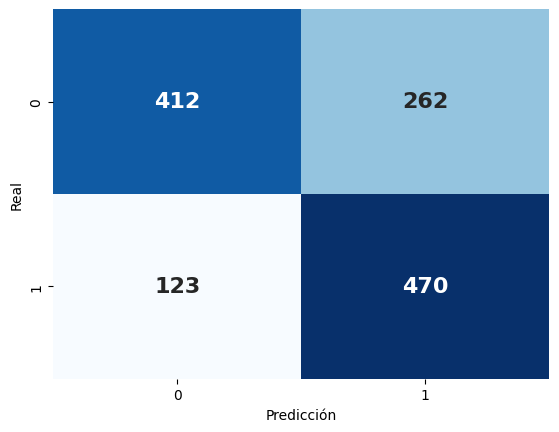
\includegraphics[width=\linewidth]{figures/decision_tree_tuned_cm.png}
    \caption{Árbol de decisión (ajustado)}
    \label{fig:cm-tree}
  \end{subfigure}\hfill
  \begin{subfigure}[t]{0.32\linewidth}
    \centering
    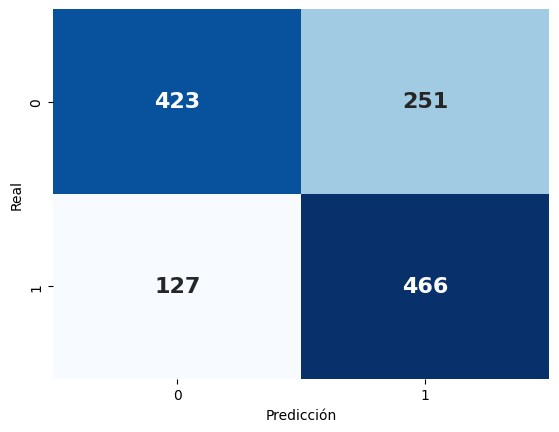
\includegraphics[width=\linewidth]{figures/logistic_cm.png}
    \caption{Regresión logística}
    \label{fig:cm-log}
  \end{subfigure}\hfill
  \begin{subfigure}[t]{0.32\linewidth}
    \centering
    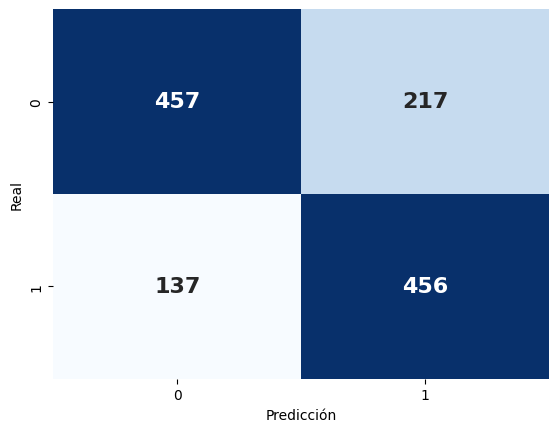
\includegraphics[width=\linewidth]{figures/ebm_cm.png}
    \caption{GAM / EBM}
    \label{fig:cm-gam}
  \end{subfigure}
  \caption{Comparativa de matrices de confusión normalizadas (0–1) para los tres modelos. El EBM presenta la mayor proporción de verdaderos positivos y falsos negativos reducidos.}
  \label{fig:cm-compare}
\end{figure}

\paragraph{Lectura breve.}
El modelo \textbf{DecisionTree (baseline)} mostró un rendimiento inicial modesto, sirviendo como referencia para validar el flujo de trabajo. 
El \textbf{DecisionTree (tuned)} logró una mejora significativa, con una \textbf{5-fold CV accuracy de 0.719}, demostrando que un árbol poco profundo y bien regularizado puede alcanzar una generalización estable.

La \textbf{Regresión Logística} ofreció un rendimiento muy equilibrado (\textbf{Train = 0.732, 5-fold = 0.702}), mostrando coeficientes coherentes con la interpretación esperada: la edad y el empleo estable reducen la probabilidad de reincidencia, mientras que el número de antecedentes la incrementa. 

Por último, el modelo \textbf{aditivo (GAM / EBM)} se consolidó como el más robusto del estudio (\textbf{Train = 0.748, 5-fold = 0.723}), manteniendo una diferencia mínima entre entrenamiento y validación. Este comportamiento indica una alta capacidad de generalización, combinando explicabilidad global (curvas de efecto) con consistencia local en las predicciones. A nivel de error, el EBM reduce falsos negativos sin aumentar excesivamente los falsos positivos, lo que lo posiciona como el modelo más equilibrado en rendimiento e interpretabilidad.

\section{Modelos}

\subsection{Comparación visual de los árboles}
El ajuste mediante \texttt{GridSearch} produce un árbol más \textbf{compacto} y, por tanto, \textbf{más explicable} (menos profundidad y reglas), manteniendo o mejorando ligeramente la precisión respecto al baseline. A continuación se muestran por separado ambos diagramas con la misma profundidad visualizada para facilitar la lectura.

\begin{figure}[h]
  \centering
  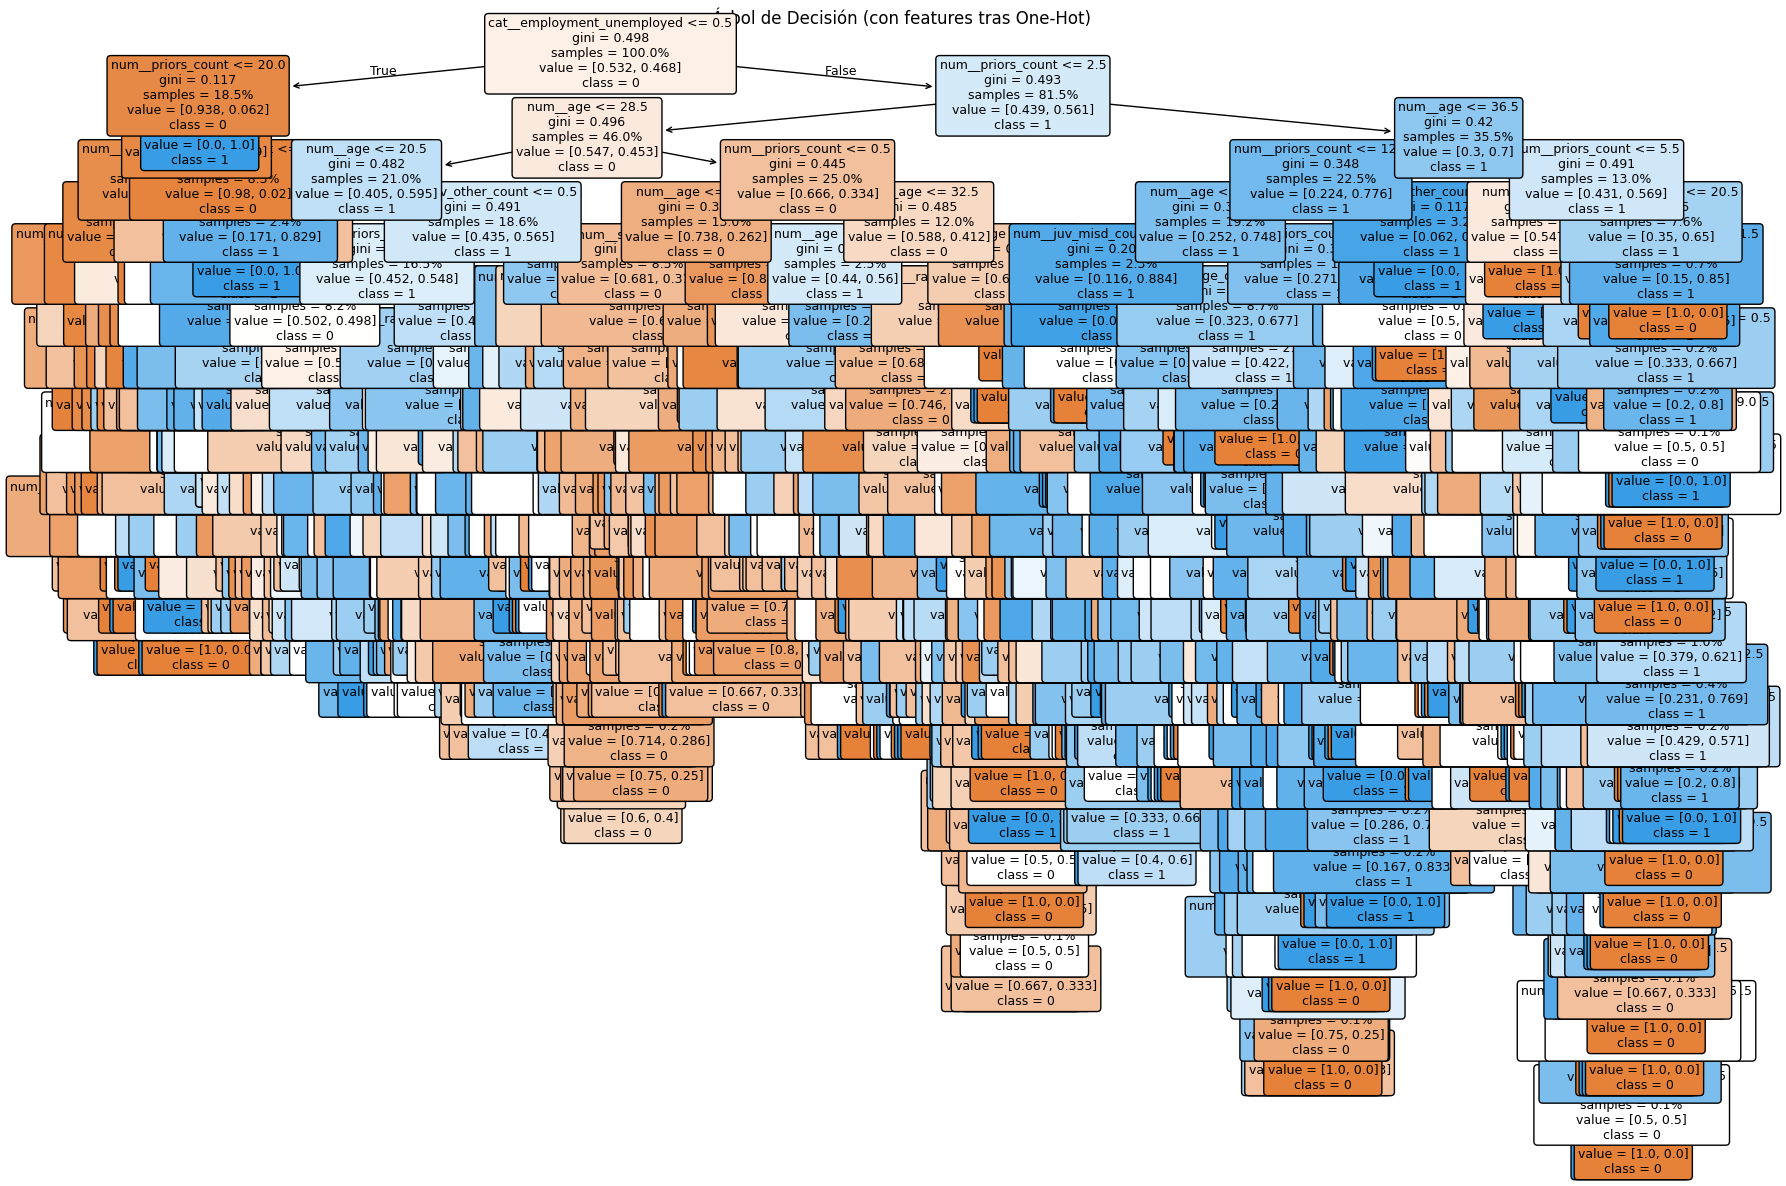
\includegraphics[width=0.92\linewidth]{figures/decision_tree_baseline_depth.png}
  \caption{Decision Tree (baseline), profundidad visualizada = 3.}
  \label{fig:tree-base}
\end{figure}

\begin{figure}[h]
  \centering
  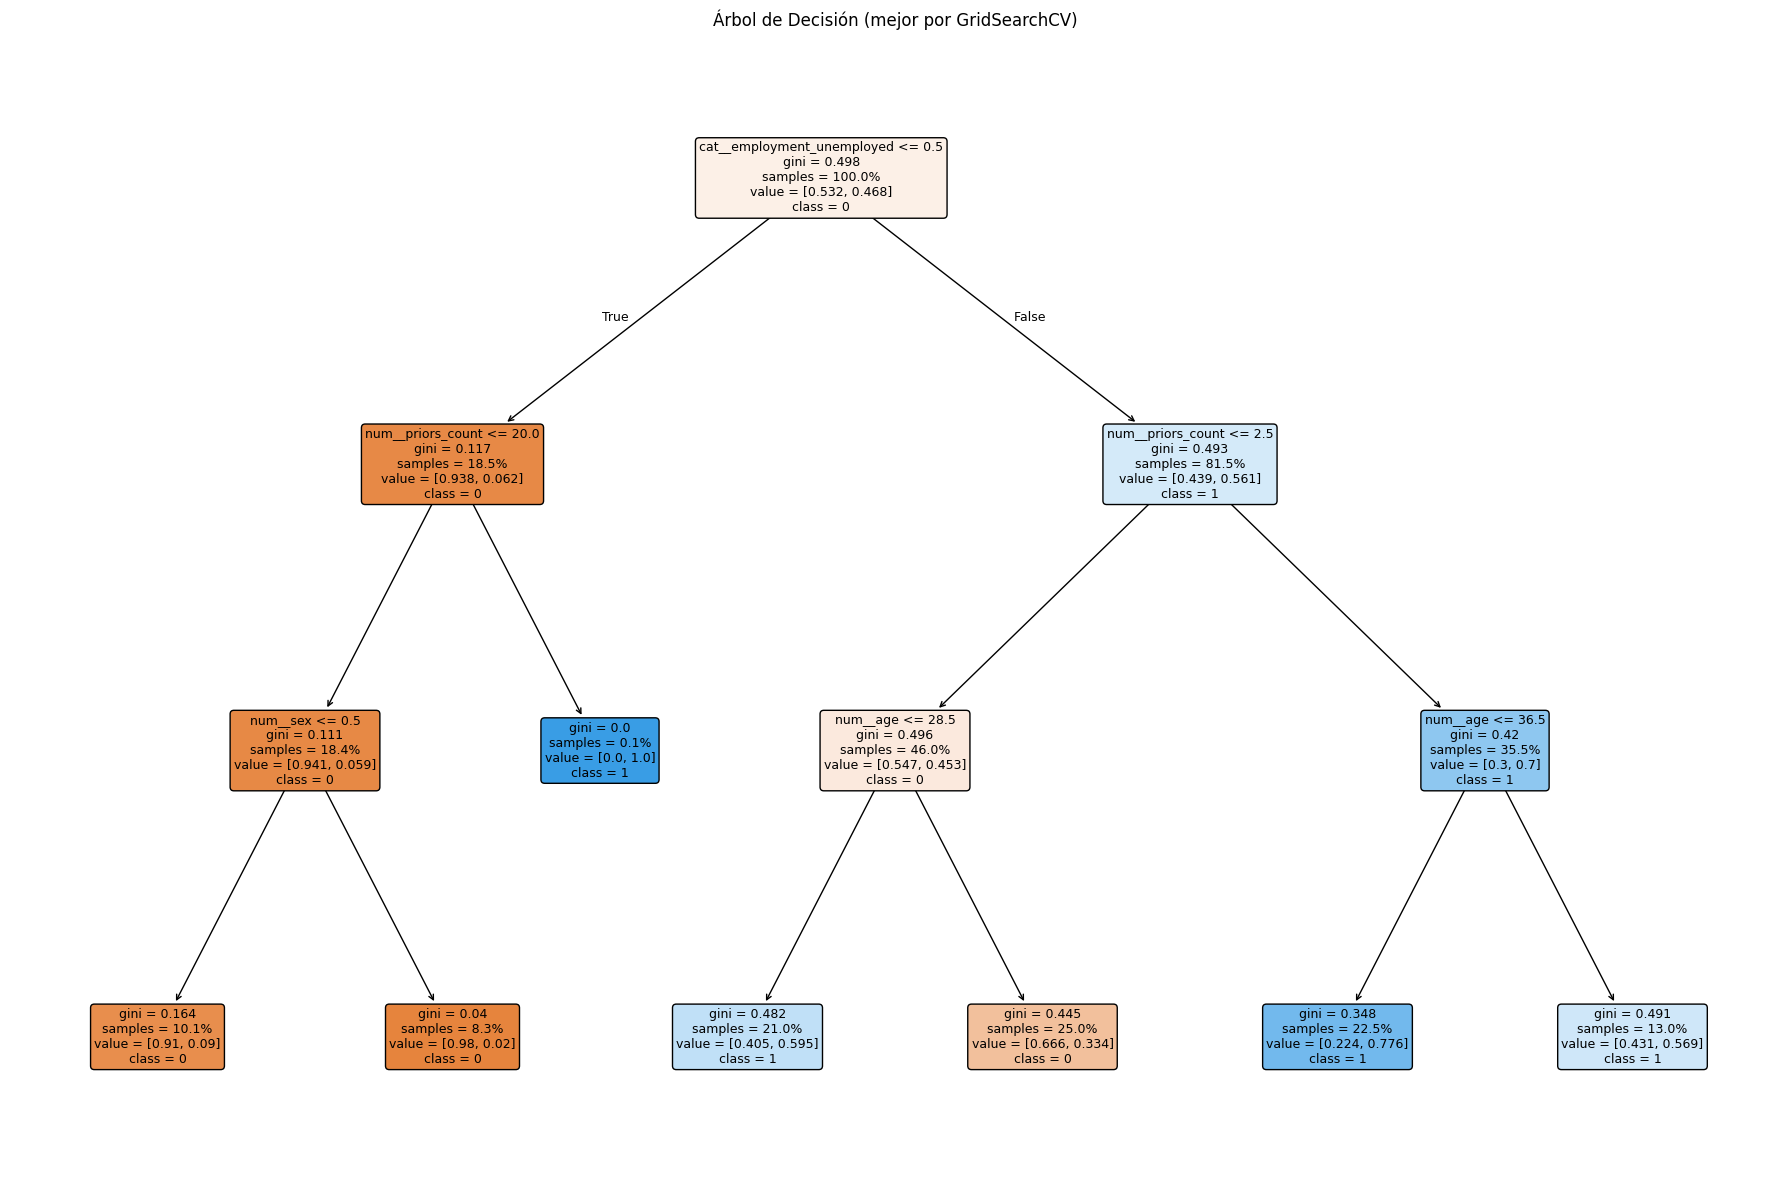
\includegraphics[width=0.92\linewidth]{figures/decision_tree_tunned_depth.png}
  \caption{Decision Tree (tuned), profundidad visualizada = 3.}
  \label{fig:tree-tuned}
\end{figure}


\begin{figure}[h]
  \centering
  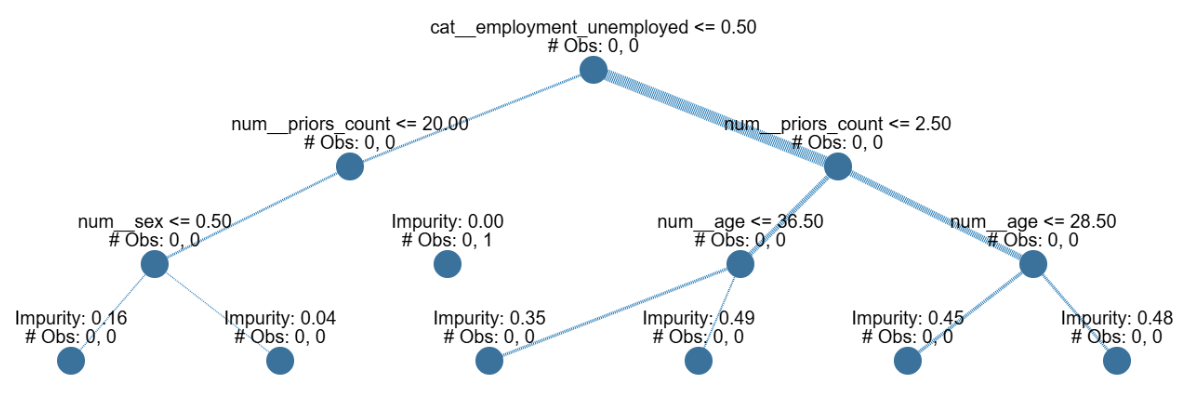
\includegraphics[width=0.92\linewidth]{figures/decision_tree_tunned_depth_global.png}
  \caption{Decision Tree (tuned) global con librería \textit{interpret}.}
  \label{fig:tree-tuned_global}
\end{figure}








\subsection{Explicación global}

El árbol ajustado concentra la decisión en pocas divisiones y umbrales sencillos, lo que facilita su lectura y comunicación. En la raíz aparece \texttt{employment\_unemployed}; a partir de ahí, \texttt{num\_priors\_count} y \texttt{age} modulan la predicción con cortes aproximados que se repiten en las ramas principales.

\paragraph{Tendencias clave.}
\begin{itemize}
  \item \textbf{Situación laboral}: si no está desempleado ($\leq 0.5$) la predicción suele inclinarse a clase 0; si está desempleado ($> 0.5$), el pronóstico depende sobre todo de antecedentes y edad.
  \item \textbf{Antecedentes} (\texttt{num\_priors\_count}): en personas empleadas, valores altos ($>20$) llevan a clase 1; en desempleados, el corte relevante baja (en torno a $2.5$).
  \item \textbf{Edad} (\texttt{age}): con pocos antecedentes, $\leq 28.5$ empuja a clase 1 y $>28.5$ a clase 0; con más antecedentes, incluso mayores de $\sim 36.5$ pueden seguir en clase 1.
  \item \textbf{Sexo}: aporta poco y solo ajusta la pureza en subramas concretas.
\end{itemize}

\paragraph{Reglas representativas (modelo ajustado).}
\vspace{-0.4em}
\begin{itemize}
  \item R1: \texttt{employment\_unemployed} $\leq 0.5$ $\land$ \texttt{num\_priors\_count} $\leq 20$ $\Rightarrow$ clase 0.
  \item R2: \texttt{employment\_unemployed} $\leq 0.5$ $\land$ \texttt{num\_priors\_count} $> 20$ $\Rightarrow$ clase 1.
  \item R3: \texttt{employment\_unemployed} $> 0.5$ $\land$ \texttt{num\_priors\_count} $\leq 2.5$: 
        si \texttt{age} $\leq 28.5$ $\Rightarrow$ clase 1; si \texttt{age} $> 28.5$ $\Rightarrow$ clase 0.
  \item R4: \texttt{employment\_unemployed} $> 0.5$ $\land$ \texttt{num\_priors\_count} $> 2.5$: 
        si \texttt{age} $\leq 36.5$ $\Rightarrow$ clase 1; si $> 36.5$ $\Rightarrow$ clase 1 (con menor pureza).
\end{itemize}

\paragraph{Comentario.}
El \texttt{GridSearch} no solo mejora ligeramente las métricas frente al baseline, sino que produce un árbol más \emph{compacto}: menos profundidad y menos reglas, por lo que se puede representar y recorrer con claridad.

% =======================
% Caso 0 — Falso positivo
% =======================
\paragraph{Explicación local (Caso 0 — Falso positivo)}.

\begin{figure}[h!]
  \centering
  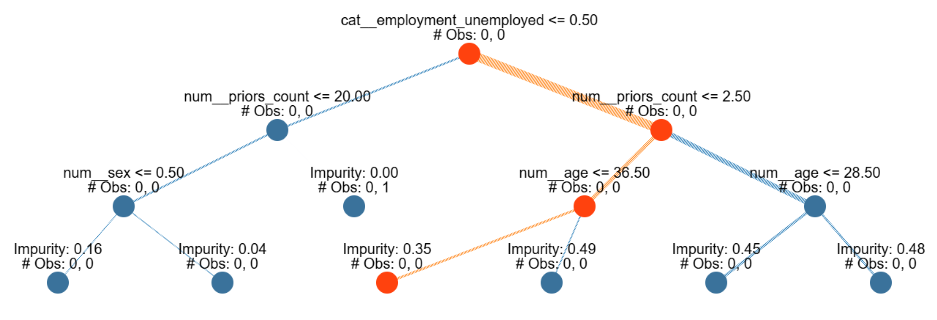
\includegraphics[width=0.92\linewidth]{figures/decision_tree_tunned_depth_local0.png}
  \caption{Decision Tree (tuned) local caso 0 con librería \textit{interpret}.}
  \label{fig:tree-tuned_local0}
\end{figure}

% --- Predicción y hoja alcanzada ---
\begin{table}[h!]
\centering
\caption{Predicción del modelo para el Caso 0.}
\label{tab:local-pred-caso0}
\small
\begin{tabular}{@{}lccc@{}}
\toprule
\textbf{Clase real} & \textbf{Clase predicha} & \textbf{PrScore} & \textbf{Decisión} \\
\midrule
0 & 1 & 0.776 & Falso positivo \\
\bottomrule
\end{tabular}
\end{table}

% --- Ruta de decisión (condiciones) ---
\begin{table}[h!]
\centering
\caption{Ruta de decisión seguida (Caso 0).}
\label{tab:local-path-caso0}
\small
\begin{tabular}{@{}cll@{}}
\toprule
\# & \textbf{Condición en el nodo} & \textbf{Rama} \\
\midrule
1 & \texttt{employment\_\_unemployed} \(> 0.5\) & Derecha \\
2 & \texttt{num\_\_priors\_count} \(\le 2.5\)   & Izquierda \\
3 & \texttt{num\_\_age} \(\le 36.5\)            & Hoja clase 1 \\
\bottomrule
\end{tabular}
\end{table}

El modelo considera que \texttt{desempleo + pocos antecedentes + edad ≤ 36.5} implica riesgo (clase 1). Sin embargo, se equivoca, pues la clase real era 0. La confianza es relativamente alta (0.776).

% =======================
% Caso 1 — Verdadero negativo
% =======================
\paragraph{Explicación local (Caso 1 — Verdadero negativo)}.

\begin{figure}[h!]
  \centering
  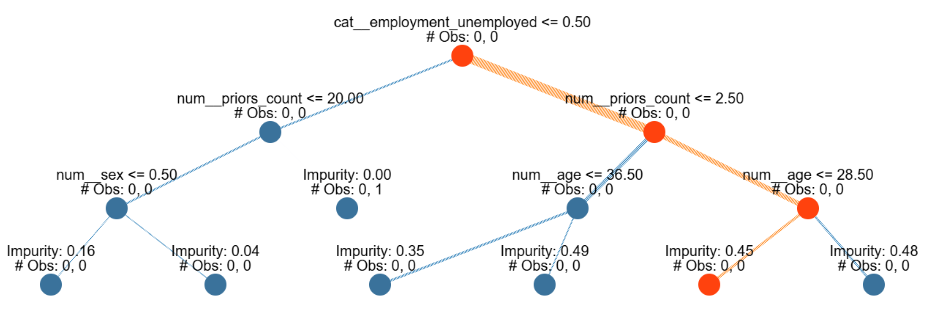
\includegraphics[width=0.92\linewidth]{figures/decision_tree_tunned_depth_local1.png}
  \caption{Decision Tree (tuned) local caso 1 con librería \textit{interpret}.}
  \label{fig:tree-tuned_local1}
\end{figure}

\begin{table}[h!]
\centering
\caption{Predicción del modelo para el Caso 1.}
\label{tab:local-pred-caso1}
\small
\begin{tabular}{@{}lccc@{}}
\toprule
\textbf{Clase real} & \textbf{Clase predicha} & \textbf{PrScore} & \textbf{Decisión} \\
\midrule
0 & 0 & 0.666 & Verdadero negativo \\
\bottomrule
\end{tabular}
\end{table}

\begin{table}[h!]
\centering
\caption{Ruta de decisión seguida (Caso 1).}
\label{tab:local-path-caso1}
\small
\begin{tabular}{@{}cll@{}}
\toprule
\# & \textbf{Condición en el nodo} & \textbf{Rama} \\
\midrule
1 & \texttt{employment\_\_unemployed} \(> 0.5\) & Derecha \\
2 & \texttt{num\_\_priors\_count} \(\le 2.5\)   & Izquierda \\
3 & \texttt{num\_\_age} \(\le 28.5\)            & Hoja clase 0 \\
\bottomrule
\end{tabular}
\end{table}

En el subgrupo de desempleados con pocos antecedentes, la condición de ser muy joven ($\leq$ 28.5) lleva al modelo a predecir bajo riesgo (clase 0), en este caso de forma correcta.

% =======================
% Caso 2 — Verdadero positivo
% =======================
\paragraph{Explicación local (Caso 2 — Verdadero positivo)}.

\begin{figure}[H]
  \centering
  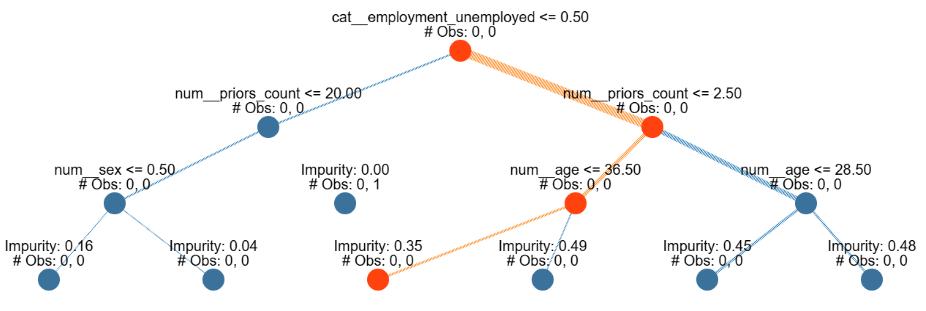
\includegraphics[width=0.92\linewidth]{figures/decision_tree_tunned_depth_local2.png}
  \caption{Decision Tree (tuned) local caso 2 con librería \textit{interpret}.}
  \label{fig:tree-tuned_local2}
\end{figure}

\begin{table}[H]
\centering
\caption{Predicción del modelo para el Caso 2.}
\label{tab:local-pred-caso2}
\small
\begin{tabular}{@{}lccc@{}}
\toprule
\textbf{Clase real} & \textbf{Clase predicha} & \textbf{PrScore} & \textbf{Decisión} \\
\midrule
1 & 1 & 0.776 & Verdadero positivo \\
\bottomrule
\end{tabular}
\end{table}

\begin{table}[H]
\centering
\caption{Ruta de decisión seguida (Caso 2).}
\label{tab:local-path-caso2}
\small
\begin{tabular}{@{}cll@{}}
\toprule
\# & \textbf{Condición en el nodo} & \textbf{Rama} \\
\midrule
1 & \texttt{employment\_\_unemployed} \(> 0.5\) & Derecha \\
2 & \texttt{num\_\_priors\_count} \(\le 2.5\)   & Izquierda \\
3 & \texttt{num\_\_age} \(\le 36.5\)            & Hoja clase 1 \\
\bottomrule
\end{tabular}
\end{table}

Mismo patrón que el Caso 0 (\texttt{desempleo + juventud relativa}), pero aquí acierta al asignar riesgo (clase 1).

% =======================
% Caso 3 — Falso negativo
% =======================
\paragraph{Explicación local (Caso 3 — Falso negativo)}.

\begin{figure}[h!]
  \centering
  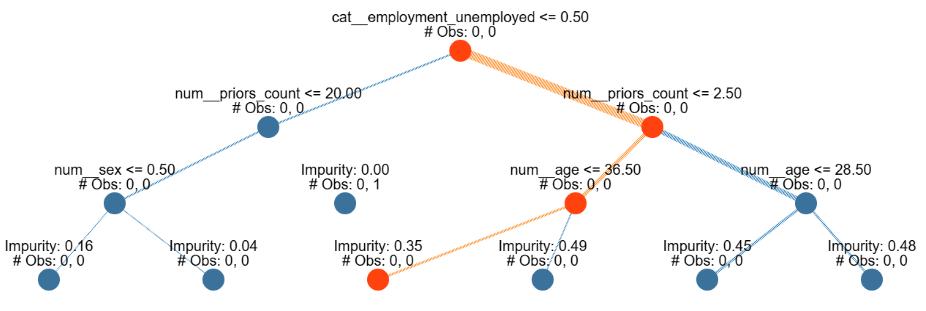
\includegraphics[width=0.92\linewidth]{figures/decision_tree_tunned_depth_local2.png}
  \caption{Decision Tree (tuned) local caso 3 con librería \textit{interpret}.}
  \label{fig:tree-tuned_local3}
\end{figure}

\begin{table}[h!]
\centering
\caption{Predicción del modelo para el Caso 3.}
\label{tab:local-pred-caso3}
\small
\begin{tabular}{@{}lccc@{}}
\toprule
\textbf{Clase real} & \textbf{Clase predicha} & \textbf{PrScore} & \textbf{Decisión} \\
\midrule
1 & 0 & 0.666 & Falso negativo \\
\bottomrule
\end{tabular}
\end{table}

\begin{table}[h!]
\centering
\caption{Ruta de decisión seguida (Caso 3).}
\label{tab:local-path-caso3}
\small
\begin{tabular}{@{}cll@{}}
\toprule
\# & \textbf{Condición en el nodo} & \textbf{Rama} \\
\midrule
1 & \texttt{employment\_\_unemployed} \(> 0.5\) & Derecha \\
2 & \texttt{num\_\_priors\_count} \(\le 2.5\)   & Izquierda \\
3 & \texttt{num\_\_age} \(\le 28.5\)            & Hoja clase 0 \\
\bottomrule
\end{tabular}
\end{table}

La misma subregla que el Caso 1 (joven, pocos antecedentes, desempleado) lleva a clasificar como bajo riesgo, pero en este caso el individuo sí era de clase 1. Se observa una tendencia del árbol a subestimar riesgo en este perfil.

% =======================
% Caso 4 — Verdadero negativo
% =======================
\paragraph{Explicación local (Caso 4 — Verdadero negativo)}.
\begin{figure}[H]
  \centering
  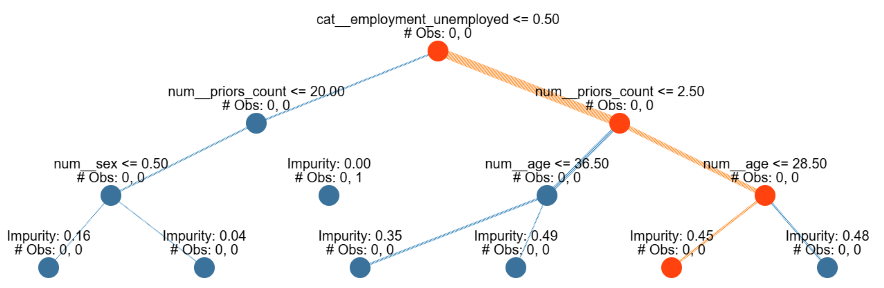
\includegraphics[width=0.92\linewidth]{figures/decision_tree_tunned_depth_local4.png}
  \caption{Decision Tree (tuned) local caso 4 con librería \textit{interpret}.}
  \label{fig:tree-tuned_local4}
\end{figure}
\begin{table}[H]
\centering
\caption{Predicción del modelo para el Caso 4.}
\label{tab:local-pred-caso4}
\small
\begin{tabular}{@{}lccc@{}}
\toprule
\textbf{Clase real} & \textbf{Clase predicha} & \textbf{PrScore} & \textbf{Decisión} \\
\midrule
0 & 0 & 0.666 & Verdadero negativo \\
\bottomrule
\end{tabular}
\end{table}

\begin{table}[H]
\centering
\caption{Ruta de decisión seguida (Caso 4).}
\label{tab:local-path-caso4}
\small
\begin{tabular}{@{}cll@{}}
\toprule
\# & \textbf{Condición en el nodo} & \textbf{Rama} \\
\midrule
1 & \texttt{employment\_\_unemployed} \(> 0.5\) & Derecha \\
2 & \texttt{num\_\_priors\_count} \(\le 2.5\)   & Izquierda \\
3 & \texttt{num\_\_age} \(\le 28.5\)            & Hoja clase 0 \\
\bottomrule
\end{tabular}
\end{table}


El patrón “desempleado, pocos antecedentes, edad baja” vuelve a dar clase 0, esta vez de forma correcta.


\section{Discusión}

\subsection*{Rendimiento}
El modelo ajustado mejora frente al baseline: \textbf{Accuracy} de $\sim$0.66 $\rightarrow$ $\sim$0.70 y subida en \textbf{F1 (macro)}. La \textbf{5-fold CV} (0.719) es coherente con esa ganancia, por lo que no parece un efecto aleatorio. A nivel de errores, se reducen falsos negativos sin un aumento desmedido de falsos positivos.

\subsection*{Interpretabilidad}
El árbol resultante es \textbf{más compacto} (poca profundidad y menos reglas), se puede dibujar y leer de arriba a abajo, y las primeras decisiones (\texttt{employment\_unemployed} $\rightarrow$ \texttt{priors\_count} $\rightarrow$ \texttt{age}) se repiten de forma clara. Las rutas locales son cortas y alineadas con esas reglas globales, lo que facilita explicar casos concretos.

\subsection*{Mejora encadenada (qué haríamos a continuación)}
\begin{enumerate}
  \item \textbf{Primero, aumentar precisión} sin romper la estructura: ampliar ligeramente la rejilla (p.\,ej., ajustes finos de \texttt{max\_depth} y \texttt{min\_samples\_leaf}) manteniendo límites de complejidad para no inflar el árbol. El objetivo es ganar algunos puntos en \textit{Accuracy}/\textit{F1} con cambios controlados.
  \item \textbf{Después, asegurar la explicabilidad}: comprobar que la profundidad, el nº de nodos/hojas y el nº de reglas se mantienen en rango “leíble”. Si creciera demasiado, aplicar poda suave (p.\,ej., \texttt{ccp\_alpha}) o volver a restricciones más estrictas. En el \emph{informe}, se pueden redondear umbrales altos para lectura; no tocar cortes sensibles como 2.5.
  \item \textbf{Por último, ajustar por clases}: con el modelo estabilizado, calibrar probabilidades y mover el umbral de decisión si se prioriza reducir falsos negativos, validándolo con \textbf{F1 (macro)} y curvas PR. La idea es afinar el equilibrio sin perder la claridad ganada.
\end{enumerate}


\section{Conclusión}

Hemos establecido una línea base interpretable con \emph{pipeline} reproducible y árbol de decisión; el modelo ajustado vía \texttt{GridSearch} resulta \textbf{más compacto} y \textbf{más legible} y mejora las métricas frente al baseline (Accuracy $\sim$0.66 $\rightarrow$ $\sim$0.70; F1 macro al alza; 5-fold CV $\sim$0.719). A nivel global, pocas reglas (empleo $\rightarrow$ antecedentes $\rightarrow$ edad) explican la mayor parte de las decisiones; a nivel local, las rutas son cortas y coherentes. De cara a mejorar sin perder explicabilidad: (i) afinar hiperparámetros para ganar algo de precisión con límites de complejidad, (ii) comprobar que el árbol sigue siendo legible, y (iii) calibrar y ajustar el umbral para reducir falsos negativos. :contentReference[oaicite:0]{index=0}

\section*{Referencias}
\begingroup
\small
\begin{itemize}
  \item Josep Gabriel Fornes Reynes; Jordi Florit Ensenyat; Juan Esteban Rincón Marín.
  \emph{XAI – Proyecto Tema 2 (Repositorio)}. GitHub.
  Disponible en: \url{https://github.com/PepBiel/IAExplicable_Proyectos/tree/main/Proyecto_Tema2}
  (acceso: Septiembre 2025).
\end{itemize}
\endgroup


% ====== Bibliografía ======
\printbibliography

% (Opcional) Apéndices
% \appendix
% \section{Apéndice: Configuración y reproducibilidad}
% \input{sections/99-appendix}

\end{document}
